\section{Qualità di processo}
\label{sec:qdp}
La capacità di raggiungere gli obiettivi prefissati è fortemente influenzata dalla qualità dei processi che portano al loro raggiungimento. Il gruppo \textit{SWEefty} utilizzerà la normativa ISO/IEC 15504 (conosciuta anche come SPICE) la quale fornisce un modello per poter giudicare lo stato di maturità di un processo.
Lo standard prevede sei diversi livelli di maturità di un processo. Di seguito vengono riportati soltanto quelli ritenuti necessari e ragionevoli per le dimensioni del \gl{progetto} da svolgere.
\begin{itemize} 
	\item \textbf{Level 1 - Performed process:}
		il  processo  viene  attuato  e  raggiunge  gli
		obiettivi prefissati ma non viene controllato rigidamente.  Gli
		attributi di tale processo sono:
		\begin{itemize}
			\item \textbf{P.A. 1.1 - Process performance:}
			capacità  di  raggiungere  i  propri
			obiettivi e produrre output identificabili.
		\end{itemize}
	\item \textbf{Level 2 - Managed process:}
		il processo è implementato, controllato, tracciato e gli output prodotti sono controllati, manutenuti e raggiungono standard prefissati.  Gli attributi di tale processo sono:
		\begin{itemize}
			\item \textbf{P.A. 2.1 - Performance management:}
				capacità  di  produrre  output che raggiungano gli obiettivi prefissati;
			\item \textbf{P.A. 2.2 - Work product management:}
				capacità di produrre output controllato e tracciato.
		\end{itemize}
	\item \textbf{Level 3 - Established process:}
		il processo viene attuato e controllato utilizzando un processo definito in grado di raggiungere gli output previsti. Gli  attributi  di  tale processo sono:
		\begin{itemize}
			\item \textbf{P.A. 3.1 - Process definition:}
			capacità  di  produrre  output  che  si
			attengano agli standard dell’ingegneria del software;
			\item \textbf{P.A. 3.2 - Process resource:}
			capacità  di  produrre  output  efficacemente utilizzando una quantità di risorse ragionevole.
		\end{itemize}
	\item \textbf{Level 4 - Predictable process:}
		il processo viene attuato con vincoli determinati  e  raggiunge  gli  obiettivi  previsti. Il processo è ben collaudato. Gli attributi di tale processo sono:
		\begin{itemize}
			\item \textbf{P.A. 4.1 - Process measurement:}
			capacità  di  utilizzare  le  misure ottenute durante l’esecuzione del processo per verificare in futuro il raggiungimento degli obiettivi prefissati;
			\item \textbf{P.A. 4.2 - Process control:}
			capacità  di  modificare  l’esecuzione  del processo in seguito ai dati raccolti.
		\end{itemize}
	\item \textbf{Level 5 - Optimizing process:}
		il processo raggiunge stabilmente i propri obiettivi ed è continuamente ottimizzato per raggiungere i futuri obiettivi.
		Gli attributi di tale processo sono:
		\begin{itemize}
			\item \textbf{P.A. 5.1 - Process change:}
			capacità di tracciare tutti i cambiamenti del processo, siano essi strutturali o di esecuzione;
			\item \textbf{P.A. 5.2 - Continuous improvement:}
			capacità di implementare le modifiche applicate.
		\end{itemize}

		Per gli attributi di processo, SPICE fornisce una scala di valutazione per misurare il loro raggiungimento:
		\begin{itemize}
			\item \textbf{N:} non posseduto (0\% - 15\%);
			\item \textbf{P:} parzialmente posseduto (16\% - 50\%);
			\item \textbf{L:} largamente posseduto (51\% - 85\%);
			\item \textbf{F:} totalmente posseduto (86\% - 100\%).
		\end{itemize}
\end{itemize}
	SWEefty utilizza il miglioramento continuo e trova nel ciclo PDCA la migliore tecnica per realizzare tale intento.
	Grazie al ciclo PDCA è possibile controllare costantemente i processi, tale ciclo è composto da quattro fasi:
	\begin{itemize}
		\item \textbf{Plan:} in questa fase si decidono gli obiettivi e i risultati che si vogliono ottenere;
		\item \textbf{Do:} si mette in atto il piano deciso nella fase precedente;	
		\item \textbf{Check:} si controllano i risultati ottenuti dalla fase Do con i risultati previsti;
		\item \textbf{Act:} si individuano le cause che possono aver interferito con il raggiungimento degli obiettivi e si decidono le azioni da intraprendere per migliorare il processo.
	\end{itemize}

	SWEefty inoltre distingue le anomalie inviduate durante la fase check in quattro diverse categorie. Ciò permette di discutere più facilmente delle correzioni da attuare durante le riunioni. Le categorie utilizzate sono quelle previste dal documento \emph{IEEE 610.12-90}:

	\begin{itemize}
	\item \textbf{Error:} differenza tra un valore o una condizione computata, osservata e misurata e il valore "teorico" corretto aspettato. (e.g: la differenza tra la stima di un costo per una determinata attività ed il suo costo effettivo);

\item \textbf{\gl{Fault}:} un processo, un'operazione o un dato definito in maniera erronea (e.g: violazione di un regola di formattazione in un documento);

	\item \textbf{Failure:} il risultato di un fault (e.g: la violazione della regola di formattazione produce un documento non valido);

	\item \textbf{Mistake:} azione umana che produce un risultato incorretto.
	\end{itemize}

	\subsection{Gestione qualità di processo}
Esistono due approcci per il controllo della qualità di processo:
\begin{itemize}
	\item \textbf{Agile:} sviluppo iterativo senza l'\gl{overhead} della documentazione. Permette uno sviluppo rapido e un'ottima capacità di adattamento in caso di modifica dei requisiti da parte del fornitore;
	
	\item \textbf{A maturità di processo:} previsto dalle buone pratiche di \gl{management}, mette al primo posto la qualità del prodotto e dei processi.
\end{itemize}
	SWEefty utilizzerà il secondo approccio in quanto più adatto ad un gruppo inesperto.
	
Dal punto di vista pratico il processo di miglioramento continuo che SWEefty utilizza (PDCA) verrà attuato nella seguente maniera:
\begin{itemize}
	\item La fase check verrà effettuata i giorni precedenti alle consegne del materiale previste dal \gl{committente} e verranno sollevate tutte le possibili problematiche riscontrate nelle due fasi precedenti (Plan, Do);
	\item La fase Act verrà effettuata a partire dal processo incrementale successivo. Successivamente si procederà nuovamente con le fasi Plan e Do.
\end{itemize}
	
	\subsection{Project assessment and control process}
		Questo processo ha lo scopo di determinare lo stato del progetto e di pianificare la sua esecuzione in maniera tale che tutte le attività procedano secondo la pianificazione e rispettino i budget imposti.
		\subsubsection{Obiettivi}
			\begin{itemize}
				\item Ogni elemento del gruppo dovrà svolgere il \gl{task} assegnatogli entro i limiti di tempo stabiliti;
				\item Le risorse utilizzate dovranno rispettare i limiti prestabiliti.
			\end{itemize}
	\subsubsection{Strategie}
	Il \emph{Project Manager} dovrà mantenere un rapporto di costante dialogo con gli esecutori di task così da rilevare prontamente eventuali ritardi e/o eccedenze nell'utilizzo delle risorse e risolvere il problema tempestivamente.
	\subsubsection{Metriche}
		\paragraph{Schedule variance} \Spazio
		\begin{itemize}
			\item \textbf{Range ottimale: }$\geq$ 0;
			\item \textbf{Range accettato: }$\geq$ 0.
		\end{itemize}
		\paragraph{Cost variance} \Spazio
		\begin{itemize}
			\item \textbf{Range ottimale: }$\geq$ 0;
			\item \textbf{Range accettato: }$\geq$ 0.
		\end{itemize}

	\subsection{Risk management process}
Questo processo ha lo scopo di identificare, analizzare, valutare, gestire e monitorare i rischi per tutta la durata del progetto.
\subsubsection{Obiettivi}
\begin{itemize}
	\item Identificare tutti i possibili rischi che possono compromettere l'esito del progetto;
	\item Sviluppare delle strategie per la prevenzione e la mitigazione degli stessi.
\end{itemize}
\subsubsection{Strategie}
SWEefty terrà sotto costante controllo tutti i rischi individuati, come specificato in \emph{Piano di Progetto v2.0.0}, così da poter agire in maniera tempestiva alla loro manifestazione.

\subsubsection{Metriche}
\paragraph{Rischi non individuati} \Spazio
	\begin{itemize}
		\item \textbf{Range ottimale: }0;
		\item \textbf{Range accettato: }0 - 4.
	\end{itemize}
    \subparagraph{Misurazioni}
    \begin{figure}[H]
    	\centering 
    	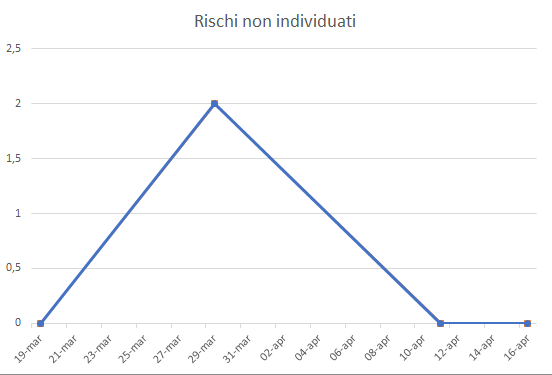
\includegraphics[width=0.7\textwidth]{Images/rischiNI.png}
    	\caption{Serie storica dei rischi non individuati}
    	\label{rischi} 
    \end{figure}

\subsection{System requirements analysis process}
Questo processo ha lo scopo di individuare i requisiti del sistema.
\subsubsection{Obiettivi}
\begin{itemize}
	\item Associare ad ogni requisito un test che verifichi il suo soddisfacimento; 
	\item Tracciare ogni requisito in modo da poter risalire alle modifiche fatte ad esso durante lo sviluppo del prodotto;
	\item Ogni requisito deve essere approvato dal committente.
\end{itemize}
\subsubsection{Strategie}
I requisiti vengono tracciati utilizzando lo strumento SWEgo.
\subsubsection{Metriche}
\paragraph{Requisiti obbligatori soddisfatti} \Spazio
\begin{itemize}
	\item \textbf{Range ottimale:} 100\%;
	\item \textbf{Range accettato:} 100\%.
\end{itemize}
\subparagraph{Misurazioni}
\begin{figure}[H]
	\centering 
	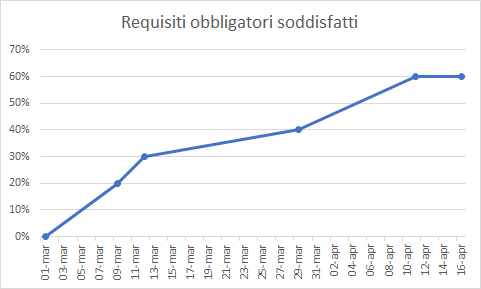
\includegraphics[width=0.7\textwidth]{Images/obbl.png}
	\caption{Serie storica dei requisiti obbligatori soddisfatti}
	\label{obbl} 
\end{figure}

\subsection{System architectural design process}
Lo scopo di questo processo è quello di associare ai requisiti del sistema una o più componenti del sistema.
		\subsubsection{Obiettivi}
		\begin{itemize}
			\item Ogni componente dovrà essere associata ad un requisito, ciò la rende tracciabile;
			\item Ottenere un sistema finale semplice con basso accoppiamento ed alta coesione;
			\item Ottenere componenti basandosi sui buoni principi della programmazione ad oggetti come il riuso del codice, l'incapsulamento e la modularizzazione.
		\end{itemize}
		\subsubsection{Strategie}
		Mantenere una tabella che associa ad ogni modulo un indice di utilità e un indice di dipendenza.
		\subsubsection{Metriche}
			\paragraph{Structural fan-in - SFIN} \Spazio
			\begin{itemize}
				\item \textbf{Range ottimale:} $\geq 2$;
				\item \textbf{Range accettato:} $\geq 0$.
			\end{itemize}
		    \subparagraph{Misurazioni}
		    \begin{figure}[H]
		    	\centering 
		    	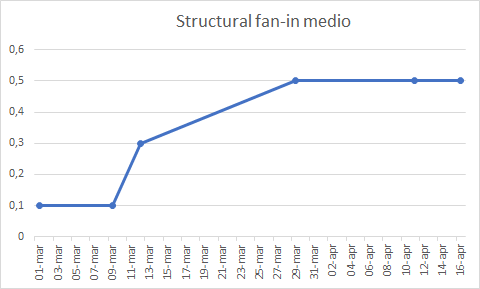
\includegraphics[width=0.7\textwidth]{Images/SFIN.png}
		    	\caption{Serie storica del Structural fan-in}
		    	\label{SFIN} 
		    \end{figure}
			\paragraph{Structural fan-out - SFOUT} \Spazio
			\begin{itemize}
				\item \textbf{Range ottimale:} 0-1;
				\item \textbf{Range accettato:} 0-5.
			\end{itemize}
		    \subparagraph{Misurazioni}
		    \begin{figure}[H]
		    	\centering 
		    	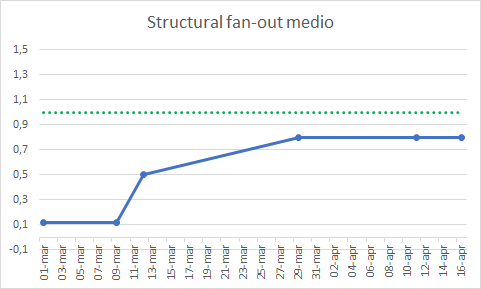
\includegraphics[width=0.7\textwidth]{Images/SFOUT.png}
		    	\caption{Serie storica del Structural fan-out}
		    	\label{SFOUT} 
		    \end{figure}
            

\subsection{System detailed design process}
Lo scopo del processo è fornire una progettazione di dettaglio del prodotto che andrà ad implementare i requisiti individuati.
		\subsubsection{Obiettivi}
		\begin{itemize}
			\item Il grado di dettaglio deve dare informazioni sufficienti alla codifica e il testing senza bisogno di ulteriori informazioni.
		\end{itemize}
		\subsubsection{Strategie}
		Le componenti individuate durante l'analisi verranno suddivise in piccole unità codificabili e testabili.
		\subsubsection{Metriche}
			\paragraph{Metodi per classe} \Spazio
			\begin{itemize}
				\item \textbf{Range ottimale:} 1-7; 
				\item \textbf{Range accettato:} 1-10.
			\end{itemize}
		    \subparagraph{Misurazioni}
		    \begin{figure}[H]
		    	\centering 
		    	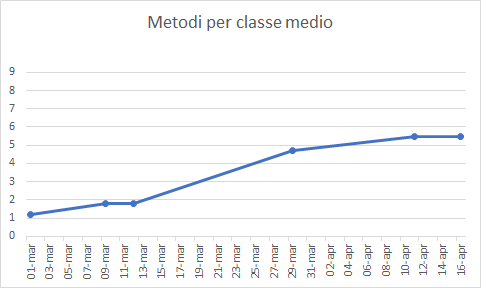
\includegraphics[width=0.7\textwidth]{Images/metodi.png}
		    	\caption{Serie storica dei metodi per classe medio}
		    	\label{metodi} 
		    \end{figure}
			\paragraph{Parametri per metodo} \Spazio
			\begin{itemize}
				\item \textbf{Range ottimale:} 0-4;
				\item \textbf{Range accettato:} 0-8.
			\end{itemize}
		    \subparagraph{Misurazioni}
		    \begin{figure}[H]
		    	\centering 
		    	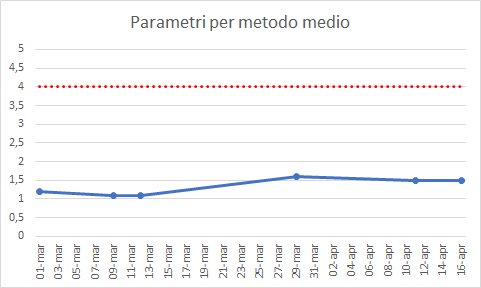
\includegraphics[width=0.7\textwidth]{Images/parametri.png}
		    	\caption{Serie storica dei parametri per metodo medio}
		    	\label{parametri} 
		    \end{figure}
			
	\subsection{Software construction process}
	\label{sub:qdp2}
	Lo scopo del processo è definire le attività principali per la produzione di unità software.
		\subsubsection{Obiettivi}
		\begin{itemize}
			\item Ottenere codice di bassa complessità per facilitarne la comprensibilità e la verifica;
			\item Ottenere codice manutenibile;
			\item Minimizzare gli sdoppiamenti di flusso.
		\end{itemize}
		\subsubsection{Strategie}
		Mantenere una bassa complessità del codice durante la stesura ed implementare al più presto dei test che ne verifichino il corretto funzionamento.
		\subsubsection{Metriche}
			\paragraph{Complessità ciclomatica} \Spazio
			\begin{itemize}
				\item \textbf{Range ottimale:} 1-10;
				\item \textbf{Range accettato:} 1-15.
			\end{itemize}
		    \subparagraph{Misurazioni}
		    \begin{figure}[H]
		    	\centering 
		    	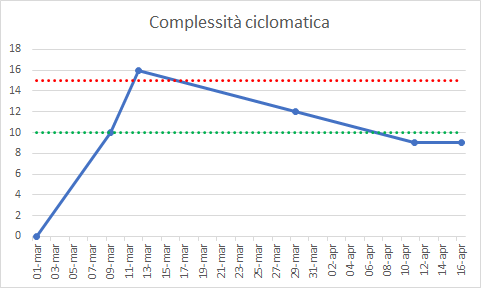
\includegraphics[width=0.7\textwidth]{Images/ciclo.png}
		    	\caption{Serie storica della complessità ciclomatica media}
		    	\label{ciclo} 
		    \end{figure}
			\paragraph{Linee di codice per linee di commento} \Spazio
			\begin{itemize}
				\item \textbf{Range ottimale:} $\geq30$;
				\item \textbf{Range accettato:} $\geq25$.
			\end{itemize}
		    \subparagraph{Misurazioni}
		    \begin{figure}[H]
		   	\centering 
		    	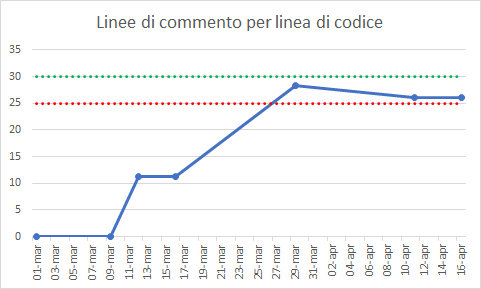
\includegraphics[width=0.7\textwidth]{Images/comm.png}
		    	\caption{Serie storica delle linee di codice per linee di commento}
		    	\label{comm} 
		    \end{figure}
			\paragraph{Halstead difficulty per-function} \Spazio
			\begin{itemize}
				\item \textbf{Range ottimale:} 0-15;
				\item \textbf{Range accettato:} 0-25.
			\end{itemize}
		\subparagraph{Misurazioni}
		\begin{figure}[H]
			\centering 
			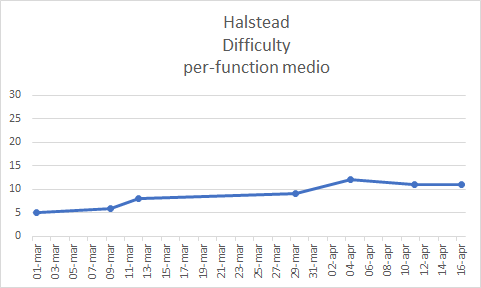
\includegraphics[width=0.7\textwidth]{Images/H-difficulty.png}
			\caption{Serie storica del Halstead Difficulty per-function}
			\label{diff} 
		\end{figure}
			\paragraph{Halstead volume per-function} \Spazio
			\begin{itemize}
			\item \textbf{Range ottimale:} 20-1000;
			\item \textbf{Range accettato:} 20-1500.
			\end{itemize}
		    \subparagraph{Misurazioni}
		    \begin{figure}[H]
		    	\centering 
		    	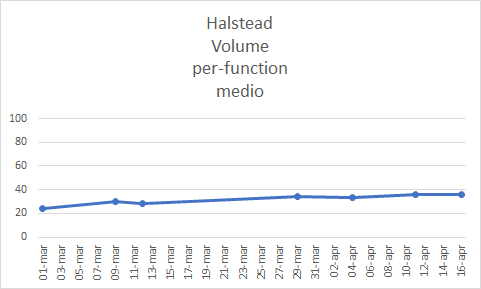
\includegraphics[width=0.7\textwidth]{Images/H-volume.png}
		    	\caption{Serie storica del Halstead Volume per-function}
		    	\label{vol} 
		    \end{figure}
			\paragraph{Halstead effort per-function} \Spazio
			\begin{itemize}
				\item \textbf{Range ottimale:} 0-300;
				\item \textbf{Range accettato:} 0-400.
			\end{itemize}
		\subparagraph{Misurazioni}
		\begin{figure}[H]
			\centering 
			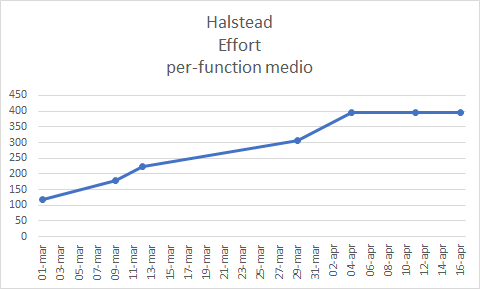
\includegraphics[width=0.7\textwidth]{Images/H-effort.png}
			\caption{Serie storica del Halstead effort per-function}
			\label{eff} 
		\end{figure}
			\paragraph{Indice di manutenibilità}  \Spazio
			\begin{itemize}
				\item \textbf{Range ottimale:} 120-171;
				\item \textbf{Range accettato:} 100-171.
			\end{itemize}
		    \subparagraph{Misurazioni}
		    \begin{figure}[H]
		    	\centering 
		    	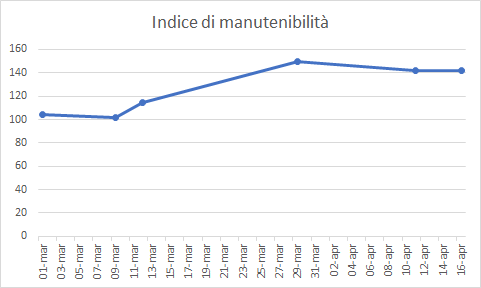
\includegraphics[width=0.7\textwidth]{Images/indicedim.png}
		    	\caption{Serie storica dell'indice di manutenibilità}
		    	\label{indicedim} 
		    \end{figure}

	\subsection{Software documentation management process}
	\label{sub:qdp3}
	
	Lo scopo del processo è quello di produrre e manutenere le informazioni sul software.
		\subsubsection{Obiettivi}
		\begin{itemize}
			\item Ottenere una documentazione comprensibile;
			\item Mantenere la documentazione aggiornata allo stato attuale del progetto.
		\end{itemize}
		\subsubsection{Strategie}
		Mantenere un diario delle modifiche e la versione del documento, inoltre per semplificare la comprensione dei documenti viene fornito un glossario che spiega il significato dei termini tecnici. 
		\subsubsection{Metriche}
			\paragraph{Indice gulpease} \Spazio
			\begin{itemize}
				\item \textbf{Range ottimale:} 50-100;
				\item \textbf{Range accettato:} 40-100.
			\end{itemize}
            \subparagraph{Misurazioni}
            \begin{figure}[H]
            	\centering 
            	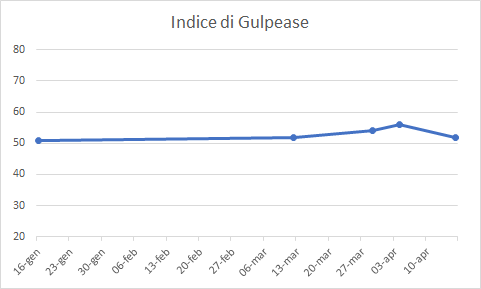
\includegraphics[width=0.7\textwidth]{Images/Gulpease.png}
            	\caption{Serie storica dell'indice di gulpease medio}
            	\label{gul} 
            \end{figure}
	\subsection{Software verification process}
	Lo scopo del processo è di verificare che tutte le componenti del sistema soddisfino completamente i requisiti ad esse correlate.
		\subsubsection{Obiettivi}
		\begin{itemize}
			\item Verificare che le varie componenti abbiano il comportamento desiderato;
			\item Utilizzare l'inspection per la verifica del codice;
			\item Automatizzare il più possibile i test dinamici.
		\end{itemize}
		\subsubsection{Strategie}
		Stilare una checklist per poi effettuare inspection su documenti e codice.
		\subsubsection{Metriche}
			\paragraph{Branch coverage}  \Spazio
			\begin{itemize}
				\item \textbf{Range ottimale:} 70\%-100\%;
				\item \textbf{Range accettato:} 50\%-100\%.
		    \end{itemize}
	        \subparagraph{Misurazioni}
	        \begin{figure}[H]
	        	\centering 
	        	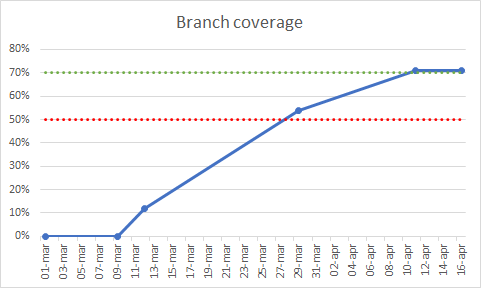
\includegraphics[width=0.7\textwidth]{Images/branch.png}
	        	\caption{Serie storica del branch coverage}
	        	\label{branch} 
	        \end{figure}
			\paragraph{Statement coverage} \Spazio
				\begin{itemize}
					\item \textbf{Range ottimale:} 70\%-100\%;
					\item \textbf{Range accettato:} 50\%-100\%.
		    	\end{itemize}
	    	    \subparagraph{Misurazioni}
	    	    \begin{figure}[H]
	    	    	\centering 
	    	    	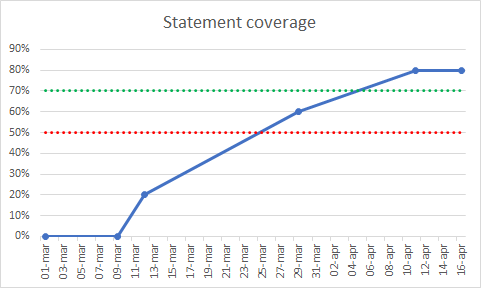
\includegraphics[width=0.7\textwidth]{Images/statement.png}
	    	    	\caption{Serie storica dello statement coverage}
	    	    	\label{statement} 
	    	    \end{figure}
